%%%%%%%%%%%%%%%%%%%%%%%%%%%%%%%%%%%%%%%%%%%%%%%%%%%%%%%%%%%%%%%%%%%%%%%%%%%%%%%
% Encoding: utf8
% Project: AIS - Exhibition ground - IS analysis and design
% Authors:
%     Libor Polčák, xpolca03@stud.fit.vutbr.cz
%     Boris Procházka, xproch63@stud.fit.vutbr.cz
%     Petr Zemek, xzemek02@stud.fit.vutbr.cz
% Description: Text of the first part of the project
%%%%%%%%%%%%%%%%%%%%%%%%%%%%%%%%%%%%%%%%%%%%%%%%%%%%%%%%%%%%%%%%%%%%%%%%%%%%%%%

\section*{Neformální specifikace}

\begin{tabular}{l p{11cm}}
	Datum interview: & 20.9.2009 \\
	Místo interview: & Výstaviště České Budějovice a.s., Husova 523, 370 21
		České Budějovice \\
	Účastnící: & Libor Polčák, Boris Procházka a Petr Zemek (za FIT VUT v~Brně),
		Ing.~Pavel Tvrdík (za Výstaviště České Budějovice)
\end{tabular} \\

Výstaviště České Budějovice (dále jen provozovatel) potřebuje informační systém
(dále jen IS), který by poskytoval informace o~expozicích jednotlivých firem.
Tento IS by měl sloužit jak návštěvníkům (informace, co jednotlivé firmy
nabízejí a kde je možné je najít), tak provozovateli (ten má k~dispozici
všechny informace), který tak bude mít všechny údaje pod kontrolou na jednom
místě a přehledně zpracované.

Základní informace jsou dostupné pro všechny návštěvníky výstaviště, kteří se
do IS nijak nepřihlašují. Mezi ně patří informace o~tom, které výstavy se
pořádají a kdy se konají. Dostupné jsou i informace o~tom, co a kde která firma
vystavuje. Také je k~dispozici kontaktní adresa, telefon a email na danou firmu
(pokud jsou tyto údaje dostupné). Je možné vyhledávat podle zvolených klíčů,
např. zobrazit pouze firmy vystavující prezentační techniku, a zobrazit
statistiky, kolik jakých firem apod.

Zaměstnanci výstaviště se do IS přihlašují pomocí přihlašovacích údajů (login a
heslo). S~IS budou pracovat dvě skupiny zaměstnanců -- vedoucí a řadoví
zaměstnanci. Obě skupiny mají na starosti správu firem, výstav a expozic.
Oproti údajům, které jsou o~firmách k~dispozici návštěvníkům, vidí zaměstnanci
výstaviště u~firem některé soukromé údaje navíc (jako je např. bankovní účet).
U~expozic je pak možné sledovat, na jakou smlouvu jsou registrované.

Vedoucí mají oproti řadovému zaměstnanci práva pro správu zaměstnanců a mohou
podepisovat smlouvy s~firmami, které se chystají na některé z~výstav
prezentovat. Dále také mohou prohlížet bližší ekonomické informace o~chodu
výstaviště. Jde například o~vybrané poplatky, seznam dlužníků apod.

Na výstavišti se vyskytuje několik pavilónů s~různou rozlohou. Každý z~pavilónů
má různé vybavení (např. občerstvení a sociální zařízení). Protože se
předpokládá stavba nových pavilónů, musí systém umožňovat jejich přidání,
případně editaci. Tuto akci může provést i běžný zaměstnanec.

Vystavující firma má přístup do IS ke svým údajům. Jednotlivé firmy se při
přístupu k~informacím jiných firem chovají jako návštěvníci, nebude tudíž možné
zjistit soukromé informace o~konkurenci. O~zaregistrování a zrušení registrace
je nutné požádat na informační lince provozovatele, která požadavek předá ke
zpracování některému ze zaměstnanců.

Pokud je firma zaregistrovaná, je možné domlouvat podmínky budoucí smlouvy.
V~momentě, kdy je smlouva hotová, je předaná vedoucímu zaměstnanci ke
schválení. K~podpisu smlouvy je nutná osobní schůzka s~provozovatelem. Tato
smlouva bude potom k~dispozici oběma stranám a nebude možné upravovat její
text. Řadový zaměstnanec nebude mít přístup k~citlivým informacím, např.
k~zaplaceným poplatkům. Ostatní firmy a běžní návštěvníci výstaviště nemají
možnost se o~této smlouvě dozvědět.

Předmětem smlouvy je poskytnutí výstavního prostoru pro několik expozic.
Smlouva se může vztahovat i na několik výstav. Před zahájením provozu je firma
povinna vyplnit v~IS všechny potřebné údaje (informace o~tom, co vystavuje a do
jakého oboru to patří). Před vložením či změnou údajů je firma povinna se
autentizovat v~IS zadáním přihlašovacího jména a hesla.

Systém by měl být jednoduchý a přehledný, aby neodradil návštěvníky od jeho
používání. Hlavním cílem je maximální usnadnění spolupráce mezi provozovatelem
a jednotlivými firmami.

Maximální částka, kterou je provozovatel ochoten věnovat do vývoje systému, je
450.000 Kč. Termín dodání a odzkoušení je do konce června, od září musí být
systém plně funkční. Kontaktní osobou bude Ing.~Tvrdík.

\pagebreak
\section*{Analýza požadavků}

Analýzou neformální specifikace jsme došli k~následujícím požadavkům na systém.

\begin{itemize}
	\item Existují dvě skupiny zaměstnanců. Některé úlohy mají společné,
	některé jsou však pouze omezeny na jednu skupinu, v~našem případě vedoucí.
	Tato skutečnost bude modelována pomocí abstraktního aktéra
	\emph{zaměstnance výstaviště}. Tento aktér bude bude mít dvě specializace
	-- \emph{vedoucí} a \emph{řadový zaměstnanec}.

	\item Vystavovatelé budou reprezentováni aktérem \emph{firma}, který může
	upravovat své údaje, včetně popisu expozic.

	\item Jelikož se zaměstnanci výstaviště a firmy musí do systému
	přihlašovat, je třeba tuto skutečnost modelovat pomocí abstraktního aktéra
	\emph{registrovaný uživatel}.

	\item Dále budou IS využívat návštěvníci výstaviště, kteří se do systému
	nepřihlašují. Budou tedy modelováni aktérem \emph{návštěvník}.

	\item Jak návštěvníci, tak registrovaní uživatelé mohou provádět některé
	společné akce. Jde například o~vyhledávání a čtení veřejných údajů. Proto
	vytvoříme zobecnění obou uživatelů IS (registrovaný uživatel a návštěvník)
	nazvané \emph{Uživatel}.
\end{itemize}

Výsledky této analýzy jsou zobrazeny na diagramu případu použití na obrázku
\ref{fig:UseCaseStage3}.

\begin{figure}[h]
	\begin{center}
		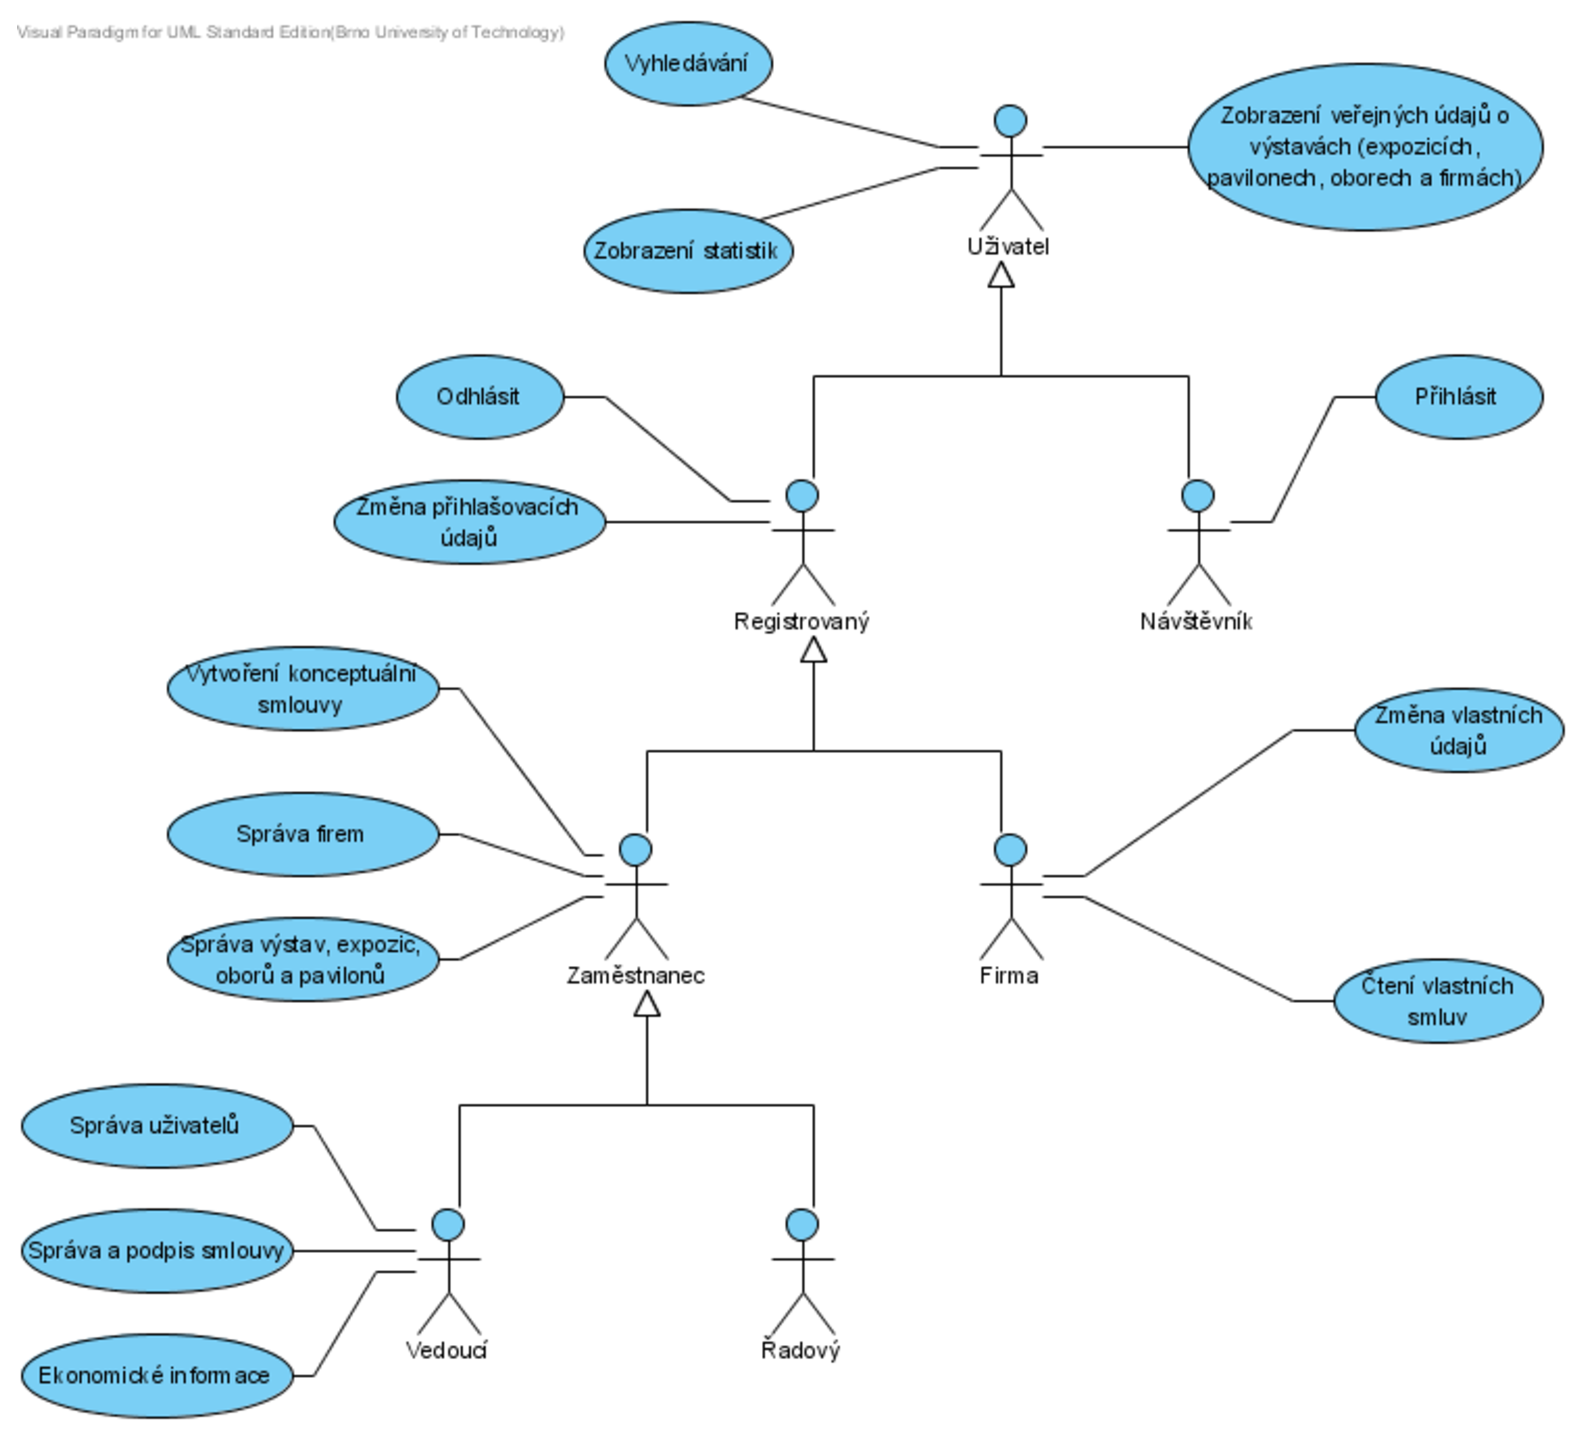
\includegraphics[width=12.5cm,keepaspectratio]{include/use_case_stage3}
	\end{center}
	\caption{Konečný diagram případů použití}
	\label{fig:UseCaseStage3}
\end{figure}

Poznámka: Případy použití, které mají ve svém názvu \uv{správa}, zahrnují
několik samostatných případů použití, ale jejich zobrazením v~diagramu by došlo
ke zhoršení přehlednosti tohoto diagramu. Typicky se jedná o~akce čti, přidej,
uprav a zruš.

\section*{Plán projektu}

Snížení míry rizik a jejich včasné předvídání je možné dosáhnout rozdělení
projektu do několika iterací. V~každé iteraci bude implementována pouze určitá
část systému, která sama o~sobě tvoří jeden funkční celek. Dle analýzy
požadavků jsme se rozhodli implementaci IS rozdělit do následujících tří
iterací.

\subsection*{1. iterace}

Již v~první iteraci budeme uvažovat různé role uživatelů. K~dosažení tohoto
cíle bude implementována možnost přihlašování a odhlašování uživatelů. S~tím
souvisí i správa uživatelů IS a jednotlivých firem, které budou na výstavišti
chtít vystavovat. V~této fázi bude do IS také přidána podpora pro uzavírání a
správu smluv s~firmami. V~této fázi však ještě nebude možné ke smlouvám
přiřazovat expozice. Diagram případů použití je ukázán na obrázku
\ref{fig:UseCaseStage1}.

\begin{figure}[h]
	\begin{center}
		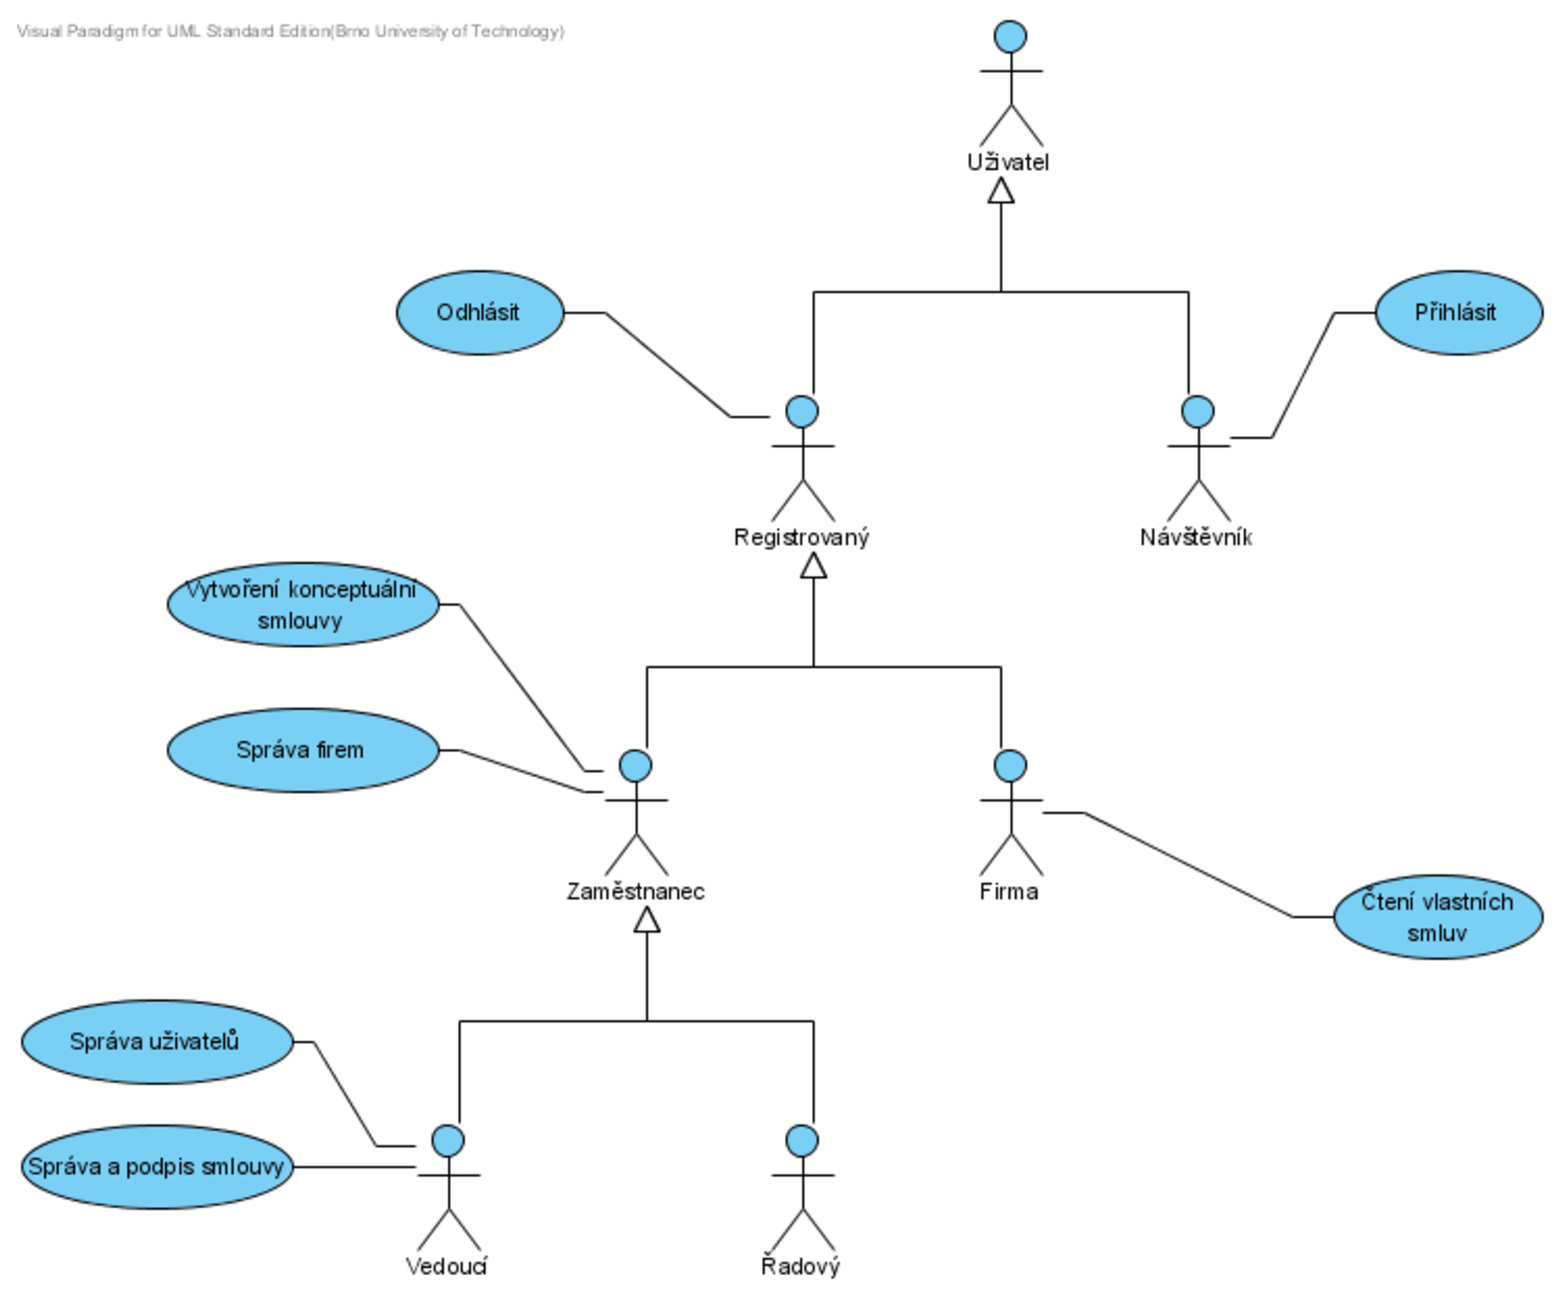
\includegraphics[width=12.5cm,keepaspectratio]{include/use_case_stage1}
	\end{center}
	\caption{Diagram případů použití po 1. iteraci}
	\label{fig:UseCaseStage1}
\end{figure}

\subsection*{2. iterace}

\begin{figure}[h]
	\begin{center}
		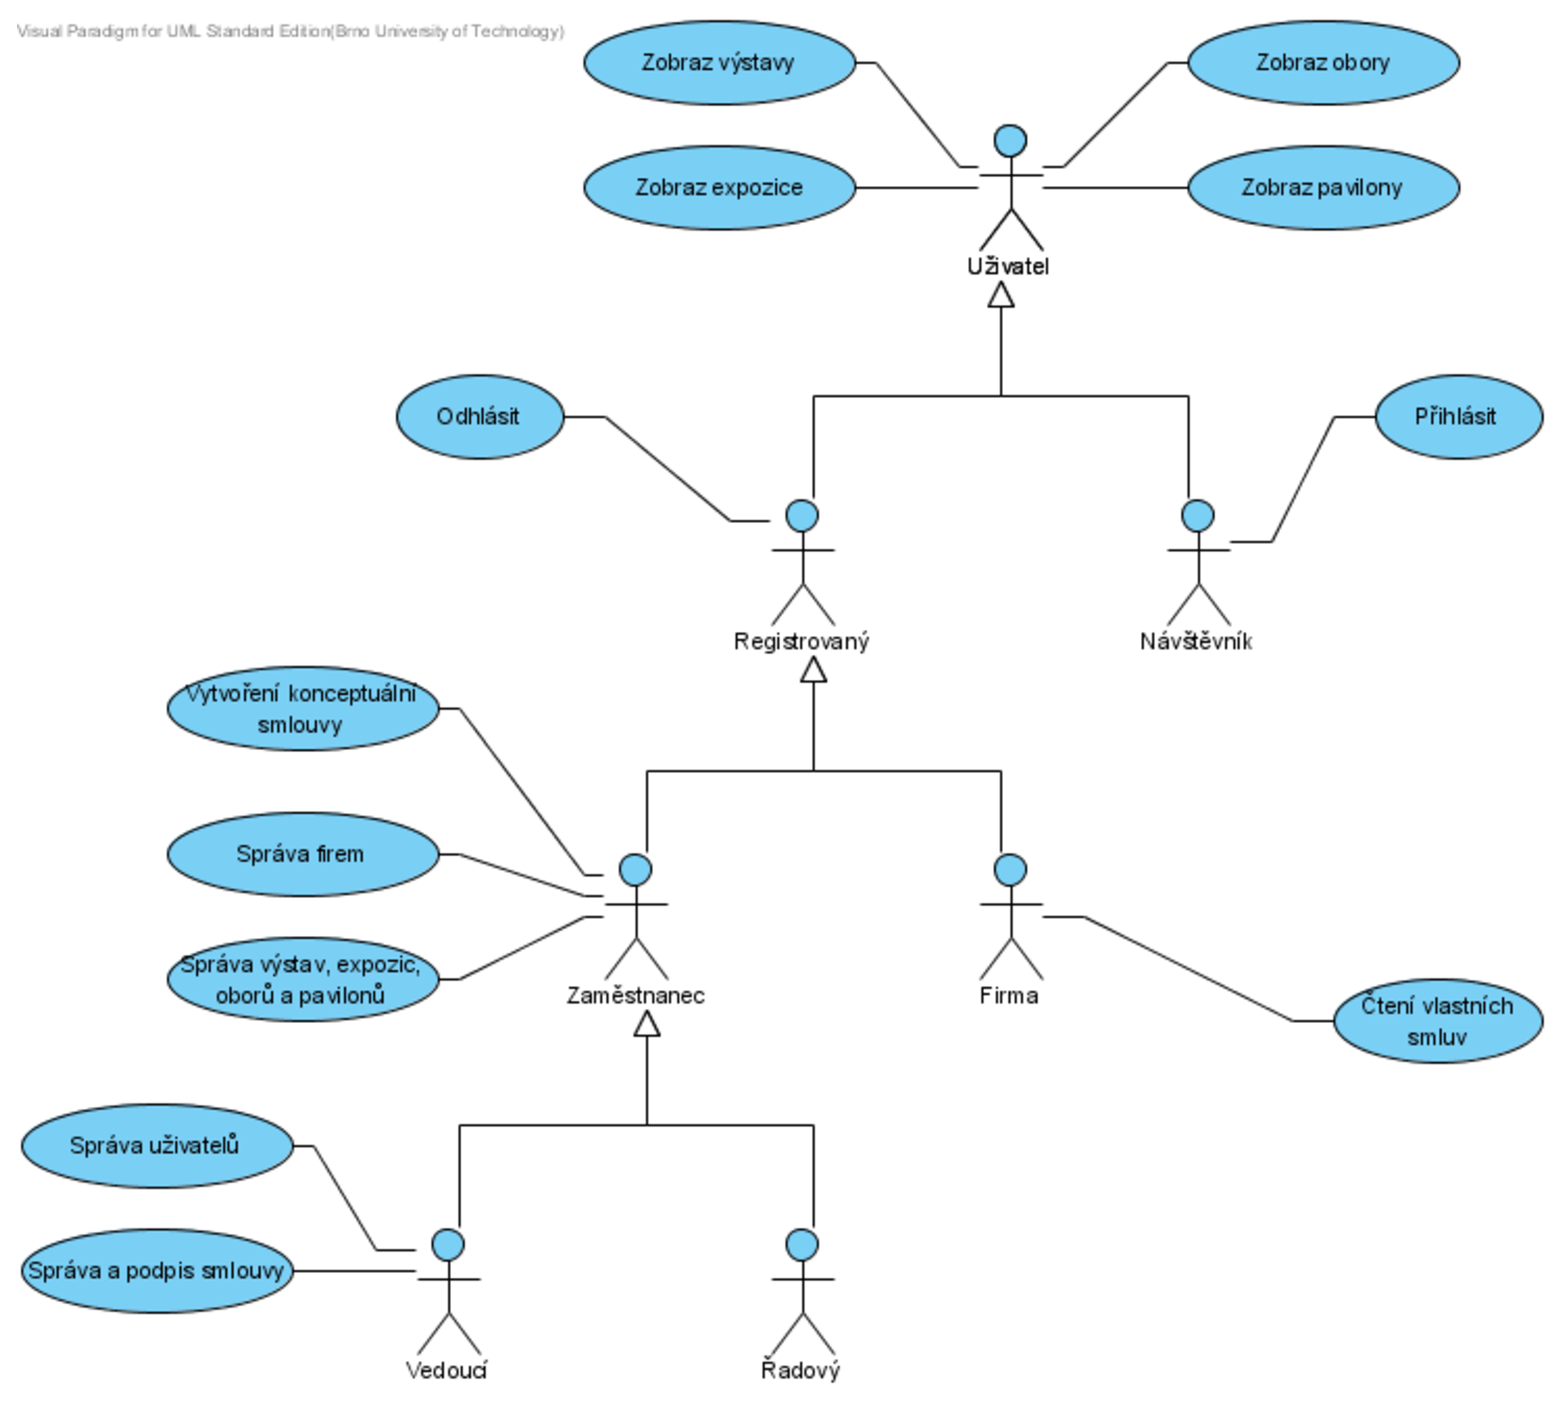
\includegraphics[width=12.5cm,keepaspectratio]{include/use_case_stage2}
	\end{center}
	\caption{Diagram případů použití po 2. iteraci}
	\label{fig:UseCaseStage2}
\end{figure}

Ve druhé iteraci implementace IS budeme modelovat ty části, které souvisí
s~vystavováním. Výstaviště obsahuje pavilóny, ve kterých se během konaných
výstav objevují různé expozice. Každá z~těchto expozic se může týkat jednoho
z~dostupných oborů. Bude implementována možnost správy těchto entit (jejich
přidávání, upravování a rušení) a zobrazování informací dostupných o~těchto
objektech. Implementace musí brát v~úvahu různé role uživatelů. Diagram případů
použití je ukázán na obrázku \ref{fig:UseCaseStage2}.

\subsection*{3. iterace}

V~závěrečné iteraci bude implementováno to, co nebylo vyhodnoceno jako vysoce
kritické. Jedná se o~změnu přihlašovacích a kontaktních údajů a získávání
informací již dostupných v~databázi, ze kterých se budou vytvářet ekonomické
(privátní) a veřejné statistiky. Dále bude umožněno vyhledávat informace
o~výstavách, expozicích a vystavujících firmách. Konečný diagram případů
použití byl ukázán na obrázku \ref{fig:UseCaseStage1}.

%%%%%%%%%%%%%%%%%%%%%%%%%%%%%%%%%%%%%%%%%%%%%%%%%%%%%%%%%%%%%%%%%%%%%%%%%%%%%%%
% vim: syntax=tex
%%%%%%%%%%%%%%%%%%%%%%%%%%%%%%%%%%%%%%%%%%%%%%%%%%%%%%%%%%%%%%%%%%%%%%%%%%%%%%%
